%%%%%%%%%%%%%%%%%%%%%%%%%%%%%%%%%%%%%%%%%
% Beamer Presentation
% LaTeX Template
% Version 2.0 (March 8, 2022)
%
% This template originates from:
% https://www.LaTeXTemplates.com
%
% Author:
% Vel (vel@latextemplates.com)
%
% License:
% CC BY-NC-SA 4.0 (https://creativecommons.org/licenses/by-nc-sa/4.0/)
%
%%%%%%%%%%%%%%%%%%%%%%%%%%%%%%%%%%%%%%%%%

%----------------------------------------------------------------------------------------
%	PACKAGES AND OTHER DOCUMENT CONFIGURATIONS
%----------------------------------------------------------------------------------------

\documentclass[
	11pt, % Set the default font size, options include: 8pt, 9pt, 10pt, 11pt, 12pt, 14pt, 17pt, 20pt
	%t, % Uncomment to vertically align all slide content to the top of the slide, rather than the default centered
	%aspectratio=169, % Uncomment to set the aspect ratio to a 16:9 ratio which matches the aspect ratio of 1080p and 4K screens and projectors
]{beamer}

\graphicspath{{Images/}{./}} % Specifies where to look for included images (trailing slash required)

\usepackage{booktabs} % Allows the use of \toprule, \midrule and \bottomrule for better rules in tables

%----------------------------------------------------------------------------------------
%	SELECT LAYOUT THEME
%----------------------------------------------------------------------------------------

% Beamer comes with a number of default layout themes which change the colors and layouts of slides. Below is a list of all themes available, uncomment each in turn to see what they look like.

%\usetheme{default}
%\usetheme{AnnArbor}
%\usetheme{Antibes}
%\usetheme{Bergen}
%\usetheme{Berkeley}
%\usetheme{Berlin}
\usetheme{Boadilla} %me gusta
%\usetheme{CambridgeUS}
%\usetheme{Copenhagen}
%\usetheme{Darmstadt}
%\usetheme{Dresden}
%\usetheme{Frankfurt}
%\usetheme{Goettingen} %dos dos
%\usetheme{Hannover} %dos dos
%\usetheme{Ilmenau}
%\usetheme{JuanLesPins}
%\usetheme{Luebeck}
%\usetheme{Madrid}
%\usetheme{Malmoe}
%\usetheme{Marburg}
%\usetheme{Montpellier}
%\usetheme{PaloAlto}
%\usetheme{Pittsburgh}
%\usetheme{Rochester} %muy flat
%\usetheme{Singapore}
%\usetheme{Szeged}
%\usetheme{Warsaw}

%----------------------------------------------------------------------------------------
%	SELECT COLOR THEME
%----------------------------------------------------------------------------------------

% Beamer comes with a number of color themes that can be applied to any layout theme to change its colors. Uncomment each of these in turn to see how they change the colors of your selected layout theme.

%\usecolortheme{albatross}
%\usecolortheme{beaver}
%\usecolortheme{beetle}
%\usecolortheme{crane}
%\usecolortheme{dolphin}
%\usecolortheme{dove}
%\usecolortheme{fly}
%\usecolortheme{lily} %default
%\usecolortheme{monarca}
%\usecolortheme{seagull}
%\usecolortheme{seahorse}
%\usecolortheme{spruce}
%\usecolortheme{whale}
%\usecolortheme{wolverine}

%----------------------------------------------------------------------------------------
%	SELECT FONT THEME & FONTS
%----------------------------------------------------------------------------------------

% Beamer comes with several font themes to easily change the fonts used in various parts of the presentation. Review the comments beside each one to decide if you would like to use it. Note that additional options can be specified for several of these font themes, consult the beamer documentation for more information.

\usefonttheme{default} % Typeset using the default sans serif font
%\usefonttheme{serif} % Typeset using the default serif font (make sure a sans font isn't being set as the default font if you use this option!)
%\usefonttheme{structurebold} % Typeset important structure text (titles, headlines, footlines, sidebar, etc) in bold
%\usefonttheme{structureitalicserif} % Typeset important structure text (titles, headlines, footlines, sidebar, etc) in italic serif
%\usefonttheme{structuresmallcapsserif} % Typeset important structure text (titles, headlines, footlines, sidebar, etc) in small caps serif

%------------------------------------------------

%\usepackage{mathptmx} % Use the Times font for serif text
\usepackage{palatino} % Use the Palatino font for serif text

\usepackage[ruled,vlined]{algorithm2e}
%\usepackage{helvet} % Use the Helvetica font for sans serif text
\usepackage[default]{opensans} % Use the Open Sans font for sans serif text
%\usepackage[default]{FiraSans} % Use the Fira Sans font for sans serif text
%\usepackage[default]{lato} % Use the Lato font for sans serif text

%----------------------------------------------------------------------------------------
%	SELECT INNER THEME
%----------------------------------------------------------------------------------------

% Inner themes change the styling of internal slide elements, for example: bullet points, blocks, bibliography entries, title pages, theorems, etc. Uncomment each theme in turn to see what changes it makes to your presentation.

%\useinnertheme{default}
\useinnertheme{circles}
%\useinnertheme{rectangles}
%\useinnertheme{rounded}
%\useinnertheme{inmargin}

%----------------------------------------------------------------------------------------
%	SELECT OUTER THEME
%----------------------------------------------------------------------------------------

% Outer themes change the overall layout of slides, such as: header and footer lines, sidebars and slide titles. Uncomment each theme in turn to see what changes it makes to your presentation.

%\useoutertheme{default}
%\useoutertheme{infolines}
%\useoutertheme{miniframes}
%\useoutertheme{smoothbars}
%\useoutertheme{sidebar}
%\useoutertheme{split}
%\useoutertheme{shadow}
%\useoutertheme{tree}
%\useoutertheme{smoothtree}

%\setbeamertemplate{footline} % Uncomment this line to remove the footer line in all slides
%\setbeamertemplate{footline}[page number] % Uncomment this line to replace the footer line in all slides with a simple slide count

%\setbeamertemplate{navigation symbols}{} % Uncomment this line to remove the navigation symbols from the bottom of all slides

%----------------------------------------------------------------------------------------
%	PRESENTATION INFORMATION
%----------------------------------------------------------------------------------------

\title[REDES NEURONALES]{Redes de funciones de base radial} % The short title in the optional parameter appears at the bottom of every slide, the full title in the main parameter is only on the title page

%\subtitle{Optional Subtitle} % Presentation subtitle, remove this command if a subtitle isn't required

\author[Luis Ballado]{Luis Ballado} % Presenter name(s), the optional parameter can contain a shortened version to appear on the bottom of every slide, while the main parameter will appear on the title slide

\institute[CINVESTAV]{CINVESTAV - UNIDAD TAMAULIPAS \\ \smallskip \textit{luis.ballado@cinvestav.mx}} % Your institution, the optional parameter can be used for the institution shorthand and will appear on the bottom of every slide after author names, while the required parameter is used on the title slide and can include your email address or additional information on separate lines

\date[\today]{\today} % Presentation date or conference/meeting name, the optional parameter can contain a shortened version to appear on the bottom of every slide, while the required parameter value is output to the title slide

%----------------------------------------------------------------------------------------

\begin{document}

%----------------------------------------------------------------------------------------
%	TITLE SLIDE
%----------------------------------------------------------------------------------------

\begin{frame}
	\titlepage % Output the title slide, automatically created using the text entered in the PRESENTATION INFORMATION block above
\end{frame}

%----------------------------------------------------------------------------------------
%	TABLE OF CONTENTS SLIDE
%----------------------------------------------------------------------------------------

% The table of contents outputs the sections and subsections that appear in your presentation, specified with the standard \section and \subsection commands. You may either display all sections and subsections on one slide with \tableofcontents, or display each section at a time on subsequent slides with \tableofcontents[pausesections]. The latter is useful if you want to step through each section and mention what you will discuss.

\begin{frame}
	\frametitle{Contenido} % Slide title, remove this command for no title
	
	\tableofcontents % Output the table of contents (all sections on one slide)
	%\tableofcontents[pausesections] % Output the table of contents (break sections up across separate slides)
\end{frame}

%----------------------------------------------------------------------------------------
%	PRESENTATION BODY SLIDES
%----------------------------------------------------------------------------------------

\section{Introducción} % Sections are added in order to organize your presentation into discrete blocks, all sections and subsections are automatically output to the table of contents as an overview of the talk but NOT output in the presentation as separate slides

%------------------------------------------------

\begin{frame}
  \frametitle{Introducción}

  \bigskip % Vertical whitespace
  
  Las redes neuronales de base radial están compuestas de tres capas: \textbf{capa de etrada, capa intermedia ó oculta}, en donde la función de activación de sus neuronas es Gaussiana, y \textbf{la capa de salida} con función de activación lineal (Perceptrón)

  \bigskip % Vertical whitespace
  
  \begin{figure}
    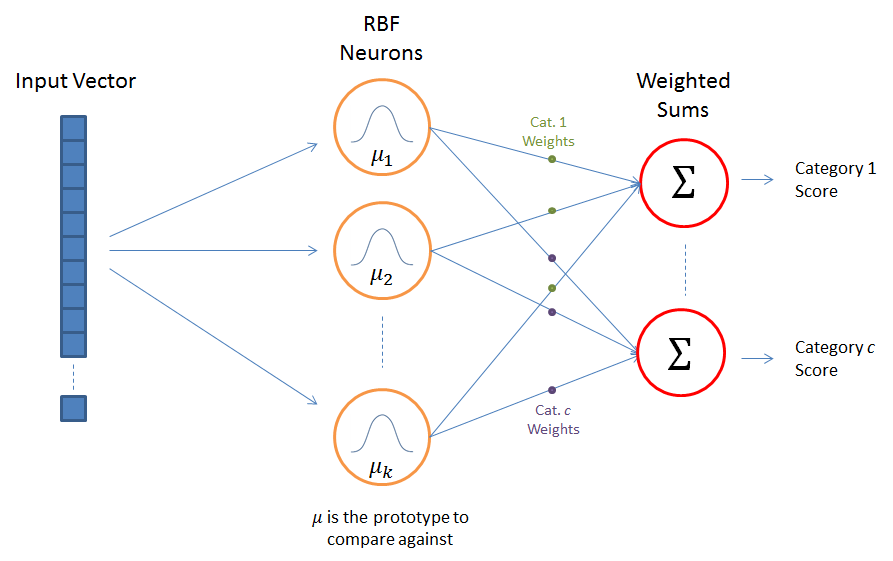
\includegraphics[width=0.6\linewidth]{architecture_simple2.png}
  \end{figure}
  
\end{frame}

\begin{frame}
  \frametitle{Introducción}

  Las funciones $\phi$ determinan las activaciones de las neuronas de la capa oculta en función de un muestra m.

  \bigskip % Vertical whitespace
  
  \textbf{Activación de las neuronas $\phi$}\\

  Utilizando una $\phi$ Gaussiana la activación de las nueronas ocultas sería: $\phi = e^{\frac{-\sum_{i=1} ^{p} (x_{i}-c_{ij})^{2}}{2\sigma^{2}_{j}}}$

  \bigskip % Vertical whitespace
  
  \begin{itemize}
  \item p: Total de características
  \item C: Centroide perteneciente a la neurona oculta j
  \item $\sum_{i=1} ^{p} (x_{i}(n)-c_{ij})^{2}$ : Distancia euclidiana del vector de entrada y el centroide $C_{j}$
  \item $\sigma^{2}$ Varianza
  \end{itemize}
\end{frame}

\begin{frame}

  \textbf{Salida de la red RBF (y)}
  \bigskip % Vertical whitespace
  \begin{center}
    $y = \sum_{i=1} ^{n} W_{i} * \phi_{i} - \theta $
  \end{center}
  \bigskip % Vertical whitespace
  Donde:
  \begin{itemize}
  \item n: neuronas en la capa oculta
  \item m: patrón de entrada (seudomuestra)
  \item $W_{i}$: pesos sinápticos que conectan las neuronas de la capa oculta y la neurona de salida y
  \item $\theta$: Umbral de la neurona de salida
  \item $\phi_{i}$: Seudomuestra
  \end{itemize}
  
\end{frame}


\begin{frame}
  En resumen:\\
  Para implementar una red RBF necesitamos:
  \bigskip % Vertical whitespace
  \begin{enumerate}
  \item Un conjunto de muestras $\rightarrow$ X (sólo para la etapa de aprendizaje)
  \item Los centroides $\rightarrow$ C
  \item El valor de la variaza $\rightarrow$ $\sigma$
  \item Las pseudomuestras $\rightarrow$ Z
  \item El valor de los pesos sinápticos $\rightarrow$ w
  \end{enumerate}
\end{frame}

\section{Paradigmas de Aprendizaje}

\begin{frame}
  
  \frametitle{El proceso de aprendizaje de la red RBF}
  Este proceso se suele llamar híbrido ya que se divide en dos fases:\\
  \bigskip % Vertical whitespace
  \begin{itemize}
  \item \textbf{Fase no supervisada}\\
    Se encarga de obtener el valor de los centroides C y la varianza $\sigma$. \\
    Para esto se suele utilizar el método \textbf{k-means}
  \item \textbf{Fase supervisada}\\
    Consiste en calcular los pesos w y umbral $\theta$ de las neuronas de la capa de salida. Para esto se suele utilizar el método de la \textbf{Regla Delta} o bien el método de la \textbf{matriz seudoinversa}
  \end{itemize}
\end{frame}

\section{El proceso de aprendizaje de la red RBF}

\begin{frame}
  Terminología:
  \begin{itemize}
  \item m: Cantidad total de muestras
  \item X: Conjunto de muestras para el \\entrenamiento $\rightarrow$ $\{X_{0}$,$X_{1}$,$X_{2}$,...,$X_{m}\}$
  \item Z: Conjunto de seudomuestras $\rightarrow$ $\{Z_{0}$,$Z_{1}$,$Z_{2}$,..,$Z_{m}\}$
  \item $\phi$: Salida de una neurona en la capa oculta
  \item y: Salida de una neurona en la capa de salida
  \item w: Pesos sinápticos que enlazan la información de las neuronas de la capa oculta con las de la capa de salida.
  \end{itemize}
\end{frame}

\begin{frame}
  \frametitle{Fase no supervisada}

  \textbf{Clasificador k-means}, ejemplo\\
  Estableciendo 2 centroides o bien dos neuronas en la capa oculta $\phi_{1}$, $\phi_{2}$:

  \begin{figure}
    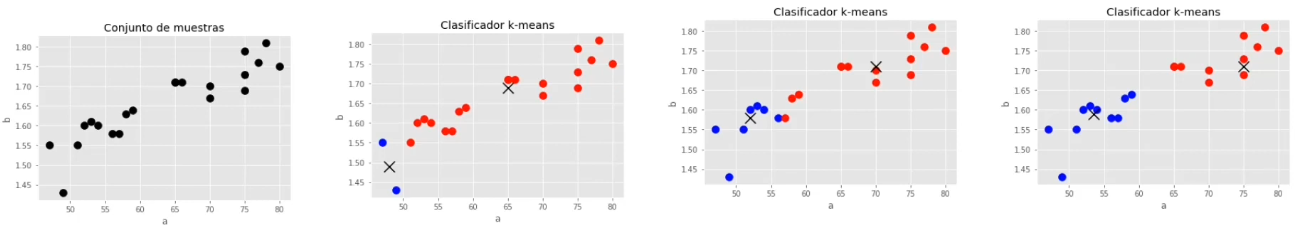
\includegraphics[width=1.0\linewidth]{kmeans.png}
  \end{figure}
  
\end{frame}

\begin{frame}
  \frametitle{Obtener pseudomuestras}

  Una vez obtenidos los valores de centroides y varianza:

  \bigskip % Vertical whitespace
  
  Generar pseudomuestras\\
  \begin{itemize}
  \item Obtener el conjunto de muestras X
  \item Generar la salida de las neuronas en la capa oculta por cada muestra del conjunto X
    \[\phi_{j}=e^{\frac{-\sum_{i=1} ^{p} (x_{i}-c_{ij})^{2}}{2\sigma^{2}_{j}}}\]

  \item $z_{i}$: Seudomuestra $\rightarrow$
    $ \begin{pmatrix}
    \phi_{1} \\
    \phi_{2} 
  \end{pmatrix}  $
  \item Z: Seudomuestras $\rightarrow$ $\{Z_{0}$,$Z_{1}$,$Z_{2}$,...,$Z_{m}\}$
  \end{itemize}
\end{frame}

\begin{frame}
  \frametitle{Método por Matriz pseudoinversa}
  Debido a que la salida de la red depende linealmente de los pesos, es posible proporcionar una solución directa con lo siguiente:
  \[ w = G^{+} * S \rightarrow (G^{t}*G)^{-1} * G^{t} * S\]

  Donde:\\
  $(G^{t} * G)^{-1} * G^{t}$, es la matriz pseudoinversa de G\\
  $G^{t}$, es la matriz transpuesta de G\\
  G, es una matriz de tamaño ($X^{m}$,$n_{oc}$) que contiene las activaciones de las neuronas de la capa oculta pero los patrones de entrada\\
  S, es la matriz de salidas deseadas, de tamaño ($X^m$,$n_{csal}$)
  
\end{frame}

\begin{frame}
  \frametitle{Representación}
  El indice superior m indica el número de muestras de aprendizaje
  \begin{figure}
    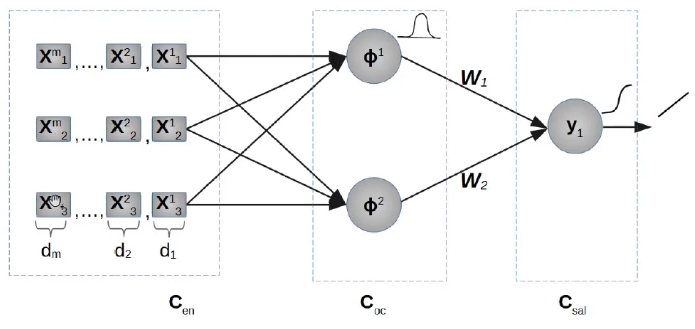
\includegraphics[width=0.7\linewidth]{rbradial.png}
  \end{figure}
  $G= \begin{pmatrix}
    \phi_{1}^{1} \phi_{1}^{2}\\
    \phi_{2}^{1} \phi_{2}^{2}\\
    \phi_{m}^{1} \phi_{m}^{2}\\
  \end{pmatrix}  $,
  $S= \begin{pmatrix}
    d_{1}\\
    d_{2}\\
    d_{m}\\
  \end{pmatrix}$,
  $w=\begin{pmatrix}
  w_{1}\\
  w_{2}\\
  \end{pmatrix}$
\end{frame}

\begin{frame}
  \frametitle{}
  Suponiendo que se tienen los siguientes valores de G y S:
  \[G= \begin{pmatrix}
    1 1\\
    1 2\\
    1 3\\
  \end{pmatrix},
  S = \begin{pmatrix}
    2\\
    2\\
    4\\
  \end{pmatrix}\]\\
  \bigskip % Vertical whitespace
  Paso 1:\\
  
  Calcular $(G^{t} * G)$
  
  \bigskip % Vertical whitespace

  \[P_{1}= \begin{pmatrix}
    1 1 1\\
    1 2 3\\
  \end{pmatrix}
  \begin{pmatrix}
    1 1\\
    1 2\\
    1 3\\
  \end{pmatrix} =
  \begin{pmatrix}
    3 6\\
    6 14\\
  \end{pmatrix}\]
  
  
\end{frame}

%------------------------------------------------
\begin{frame}
  Paso 2:

  \bigskip % Vertical whitespace

  Calcular la inversa $(G^{t}*G)^{-1} \rightarrow (P_{1}^{-1})$\\

  Utilizado el método de Gauss-Jordan:\\

  $R1*\frac{1}{3} = \begin{pmatrix}
    1  2 | \frac{1}{3} 0\\
    6 14 | 0 1\\
  \end{pmatrix} \rightarrow R2 - 6R1 = \begin{pmatrix}
    1 2 | \frac{1}{3} 0\\
    0 2 | -2 1\\
  \end{pmatrix} \rightarrow R1-R2 = \begin{pmatrix}
    1 0 | \frac{7}{3} -1\\
    0 2 | -2 1\\
  \end{pmatrix} \rightarrow R2 * \frac{1}{2} = \begin{pmatrix}
    1 0 | \frac{7}{3} -1\\
    0 1 | -1 \frac{1}{2}\\
  \end{pmatrix}$\\

  Entonces $(G^{t}*G)^{-1}$ es: \\
  \[P2 = \begin{pmatrix}
    \frac{7}{3} (-1)\\
    (-1) \frac{1}{2}\\
  \end{pmatrix}\]
\end{frame}
%------------------------------------------------

\begin{frame}
  \frametitle{utilizado el método de determinantes}

  \[(P_{1})^{-1} = \frac{1}{|P_{1}|}*(P_{1}^{*})^{t}\]

  Si $P_{1} = \begin{pmatrix}
    3 6\\
    6 14\\
  \end{pmatrix}$ Entonces:\\
  $|P_{1}|= \begin{pmatrix}
    3 6\\
    6 14\\
  \end{pmatrix} \rightarrow 42-36=6$
  $P_{1}^{*} = \begin{pmatrix}
    14 -6\\
    -6  3\\
  \end{pmatrix} \rightarrow (P_{1}^{*})^{t} = \begin{pmatrix}
    14 -6\\
    -6  3\\
    \end{pmatrix}$
  $\frac{1}{|P_{1}|}*(P_{1}^{*})^{t} = \frac{\begin{pmatrix} 14 -6\\-6 3\\ \end{pmatrix}}{6} \rightarrow \begin{pmatrix} \frac{7}{3} -1\\
    -1 \frac{1}{2}\\
  \end{pmatrix}$ 
\end{frame}

\begin{frame}
  Paso 3: Calcular $((G^{t}*G)^{-1}*G^{t}) \rightarrow (P_{2}*G^{t})$:\\
  
  \[P_{3} = \begin{pmatrix}
    \frac{7}{3} -1\\
    -1  \frac{1}{2}\\
  \end{pmatrix} * \begin{pmatrix}
    1 1 1\\
    1 2 3\\
  \end{pmatrix} = \begin{pmatrix}
    \frac{4}{3} \frac{1}{3} \frac{-2}{3}\\
    \frac{-1}{2} 0 \frac{1}{2}\\
  \end{pmatrix}\]\\

  Paso 4: Obtener w por medio de $P_{3}*S:$ \\

  \[ w = \begin{pmatrix}
    \frac{4}{3} \frac{1}{3}  \frac{-2}{3}\\
    \frac{-1}{2} 0  \frac{1}{2}\\
  \end{pmatrix} \begin{pmatrix}
    2\\
    2\\
    4\\
  \end{pmatrix} = \begin{pmatrix}
    \frac{2}{3}\\
    3\\
    1\\
  \end{pmatrix}
  \]\\

  Por lo tanto:   \[w = G^{+} * S = \begin{pmatrix}
    \frac{2}{3}\\
    1\\
  \end{pmatrix}\]
\end{frame}

%------------------------------------------------
\begin{frame}
  \frametitle{Aprendizaje de la red RBF, por Regla Delta}

  Paso 1 - Consiste en obtener la salida de la red $(y)$ mediante:\\

  \[ y = \sum_{i=1} ^{n} (w_{i}*\phi_{i}) - \theta\]

  Paso 2 - Consiste en corregir el valor de los pesos w dependiendo del error cometido por la red dada una muestra i:
  \[e_{i} = (d_{i}-y_{i})\]

  Evaluación: Consiste en evaluar el error global cometido por la red, y en caso de cumplir con un umbral de precisión $\epsilon$ termina el entrenamiento:

  \[e_{medio}=\frac{1}{2}(e_{i})^{2} \quad E=\frac{1}{p} \sum_{k=1} ^{p} e_{medio}\]
  
\end{frame}

\begin{frame}
  \frametitle{Regla Delta}

  Paso 1: Inicialización
  
  \bigskip % Vertical whitespace

  Tomando en cuenta que ya se realizo el proceso de generar las seudomuestras $\phi$ representadas por la matriz Z

  \bigskip % Vertical whitespace
  
  \begin{itemize}
  \item Inicializar el valor de los pesos w con valores aleatorios pequeños
    
    \bigskip % Vertical whitespace

  \item Inicializar el valor de $\theta = 1;\mu,\epsilon$ y épocas. 
  \end{itemize}\\
\end{frame}

\begin{frame}
  Paso 2: Generar la salida de la red

  \begin{itemize}

  \item Suponiendo que se tienen los siguientes valores:
    \[zi = \begin{pmatrix}
      0,5\\
      0,4\\
    \end{pmatrix}, w=\begin{pmatrix} 0,2 \quad 0,8\\ \end{pmatrix} \lambda = 0.2\]

  \item Obtener la salida de la neurona en la capa de salida (y) dada una seudomuestra $z_{i}$:
    \[I = \sum_{i=1} ^{n} (w_{i} * \phi_{i})-\theta \rightarrow (0,2 \quad 0,8)\begin{pmatrix}0,5\\0,4\\\end{pmatrix} \]\[= (0,5*0,2) + (0,4*0,8) = 0,42-1 = -0,58\]

    \item Aplicar una función de activación (tanh o sigmoide):
      \[y = tanh(I) \rightarrow tanh(-0,58) = -0,52\]
      
  \end{itemize}
\end{frame}

\begin{frame}
  \frametitle{Regla Delta}

  Paso 3: Ajustar los pesos sinápticos w

  \bigskip % Vertical whitespace
  
  \begin{itemize}
  \item Obtener el error e de la red dada una muestra $\phi$: \\
    (d-y) $\rightarrow$ (1-(-0,52)) = 1,52
  \item Obtener $\delta$: $e*\frac{\partial I}{\partial y}\rightarrow e*\frac{1}{1+tanh(y)^{2}} \rightarrow 1,52*0,81 = 1,23$
  \item Ajustar los pesos w: $w+(\lambda*\delta*\phi^{t})\rightarrow (0,2 \quad 0,8)+(0,2*1,23*(0,5 \quad 0,4))$
    \[(0,5 \quad 0,8)+(0,122 \quad 0,098) = (0,652 \quad 0,898)\]
  \item Ajustar $\theta$: $\theta + (\lambda * \delta)$
  \end{itemize}
  
\end{frame}

\begin{frame}
  Paso 4: Evaluación
  
  \bigskip % Vertical whitespace

  \begin{itemize}
  \item Evaluar el error cometido por la red por cada iteración $e_{i} = \frac{1}{2}*(d_{i}-y_{i})^{2}$

    \bigskip % Vertical whitespace
    
  \item Al termino de evaluar todas las muestras, calcular el error global:
    \[ E_{g} = \frac{1}{p} * \sum e_{i}\]
  \end{itemize}
\end{frame}

\section{Algoritmo}
\begin{frame}
  \begin{algorithm}[H]
    \algsetup{linenosize=\tiny}
  \scriptsize
    \SetAlgoLined
    Obtener el conjunto de muestras de entrenamiento $X \rightarrow \{X^1,X^2,X^3,...,X^m\}$, donde $X^{m} \rightarrow \{x_1,x_2,x_2,...x_n\}$\;
    Determinar el número de conjuntos k\;
    Dar un valor inicial aleatorio a los k centroides c, tomando las primeras k muestras de X\;
    Indicar el umbral de cambio para los centroides u\;
    \For{máx iteraciones}{
      \For{todas las muestras de X}{
        Calcular la distancia Euclidiana entre cada c y $X^{m}$\;
        Dado un vector $X^{m}$, determinar a cuál centroide c se encuentra más cercano \;
        Atribuir $X^{m}$ al grupo $\Omega^{c}$\;
      }
      Determinar el cambio de posición de cada centroide c $\rightarrow$ cambio\;
      \If{u$>$cambio}{
        terminar ciclo\;
      }
    }
    \For{todo c}{
      Calcular la variaza de cada función de activación Gaussiana usando el criterio de los minimos cuadrados:\\
      $\sigma^{2} = \frac{1}{p} \sum_{x^{k}\Epsilon\Omega^{j}} \sum_{i=1} ^{n} (X_{j} ^{k} - C_{i})^{2}$, donde p es el número de muestras \;
      
    }
    \caption{Fase no supervisada, k-means}
  \end{algorithm}
\end{frame}

\begin{frame}
  \begin{algorithm}[H]
    \algsetup{linenosize=\tiny}
  \scriptsize
    \SetAlgoLined
    Obtener las muestras de entrenamiento X\;
    Obtener las salidas deseadas para cada muestra d\;
    Inicializar los pesos w con valores aleatorios pequeños\;
    Especificar la tasa de aprendizaje $\lambda$, el número de épocas máximo y la precisión $\epsilon$ de la red\;
    \For{todas las muestras X}{
      Obtener $\phi$ de cada neurona oculta con respecto a $\Omega^{c}$ \rightarrow $\phi_{n1}$ = $e^{\frac{-\sum_{i=1 ^{n} (x_{i}(n)-c_{n1})^{2}}}{2\sigma^{2}_{c}}}$\;
      Generr seudomuestras $Z \rightarrow$ z = $\{\phi(1),\phi(2),...,\phi(n1)\}$\;
    }
    \While{$\epsilon > E$}{
      $E_{prev} = E_{g}$\;
      \For{seudomuestra de Z}{
        Obtener la salida de la red $\rightarrow y = \sum_i=1 ^{n} (\phi_{i}*w_{i})-\theta$\;
        Ajustar $w \rightarrow w + (z_{i} * \delta * \lambda)$\;
        Obtener salida de la red con los nuevos w y computar el error cuadrático medio $\rightarrow \frac{1}{2} * (d-y)$\;
      }
    }
    Obtener el error global $E_{g} \rightarrow \frac{E_{medio}}{p}$ donde p es la cantidad de muestras\;
    Obtener $E \rightarrow |(E_{g}-E_{prev})|$\;
    \caption{Fase supervisada, Perceptrón - Regla Delta}
  \end{algorithm}
\end{frame}

\begin{frame}
  \begin{algorithm}[H]
    \algsetup{linenosize=\tiny}
  \scriptsize
    \SetAlgoLined
    Obtener las muestras de entrenamiento $X^{m}$\;
    Obtener las salidas deseadas para cada muestra $d^{m}$\;
    \For{todas las muestras $X^{m}$}{
      Obtener $\phi$ de cada neurona oculta con respecto a $\Omega^{c}$ \rightarrow $\phi_{n1}$ = $e^{\frac{-\sum_{i=1 ^{n} (x_{i}(n)-c_{n1})^{2}}}{2\sigma^{2}_{c_{n1}}}}$\;
      Generr seudomuestras $G^{k} \rightarrow$ z = $\{\phi(1),\phi(2),...,\phi(n1)\}$\;
    }
    Obtener matriz de pesos $w \rightarrow G^{+} * S$\;
    \textbf{return} w\;
    \caption{Fase supervisada, Perceptrón - Regla Delta}
  \end{algorithm}
\end{frame}

\begin{frame}
  \frametitle{Arquitectura de la red para uso como aproximador de funciones}

  \begin{figure}
    \caption{Arquitectura de red neuronal de base radial}
    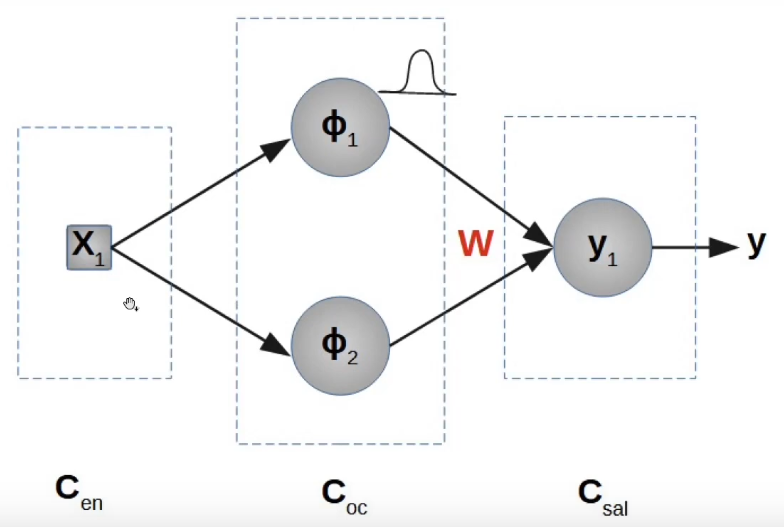
\includegraphics[width=0.6\linewidth]{last_.png}
  \end{figure}
  
  
\end{frame}

\section{Implementación Python}
\begin{frame}
  \frametitle{Implementación Python}

  Aproximador universal de funciones

  \begin{itemize}
  \item Estableciendo $\lambda = 0,015$ y un total de épocas de 5000
  \end{itemize}
  
  \begin{figure}
    \caption{Usando 1 neurona $\phi$}
    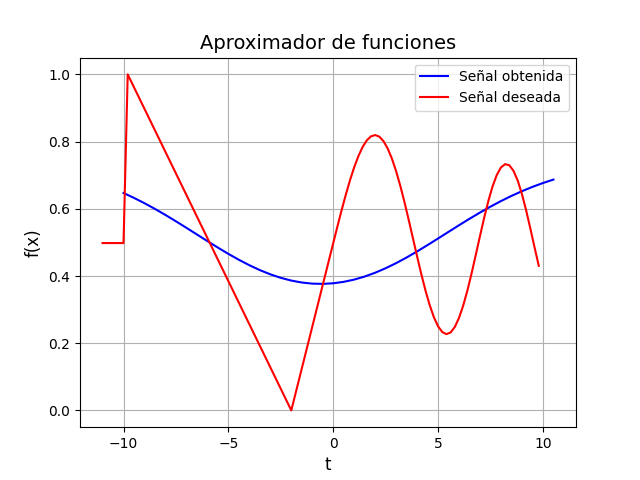
\includegraphics[width=0.6\linewidth]{1neurona.png}
  \end{figure}
  
  
\end{frame}

\begin{frame}
  \begin{figure}
    \caption{Usando 3 neuronas $\phi$}
    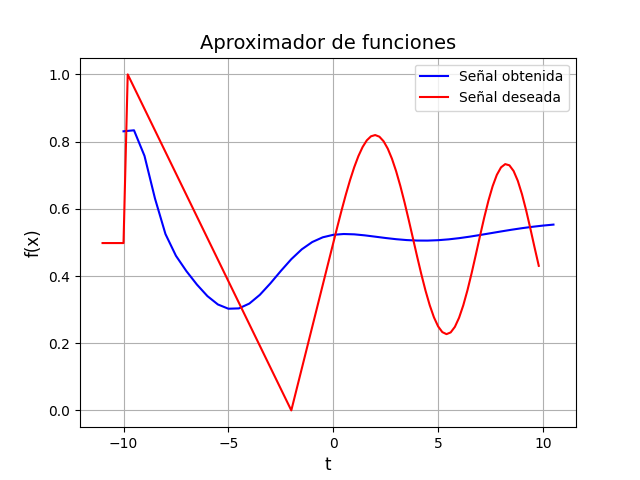
\includegraphics[width=0.6\linewidth]{3neuronas.png}
  \end{figure}
\end{frame}

\begin{frame}
  \begin{figure}
    \caption{Usando 4 neuronas $\phi$}
    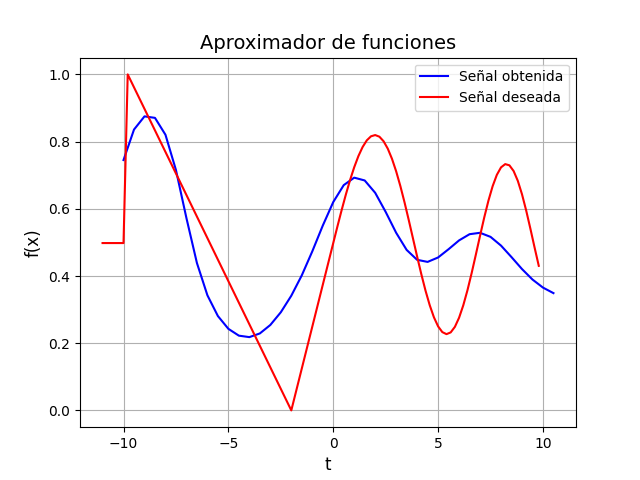
\includegraphics[width=0.6\linewidth]{4neuronas.png}
  \end{figure}
\end{frame}

\begin{frame}
  \begin{figure}
    \caption{Usando 6 neuronas $\phi$}
    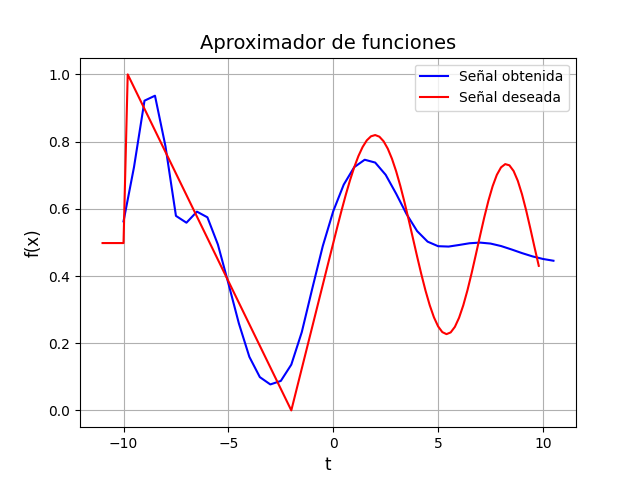
\includegraphics[width=0.6\linewidth]{6neuronas.png}
  \end{figure}
\end{frame}
%------------------------------------------------


\end{document} 
